\documentclass[11pt,a4paper]{article}

\usepackage[T1]{fontenc}
\usepackage[utf8]{inputenc}
\usepackage[romanian]{babel}
\usepackage{lmodern}
\usepackage{microtype}
\usepackage[a4paper,margin=20mm,headheight=15pt]{geometry}
\usepackage{graphicx}
\usepackage{booktabs}
\usepackage{tabularx}
\usepackage{longtable}
\usepackage{array}
\usepackage{xcolor}
\usepackage{amsmath}
\usepackage{amssymb}
\usepackage{caption}
\usepackage{subcaption}
\usepackage{float}
\usepackage{enumitem}
\usepackage{pdflscape}
\usepackage{fancyhdr}
\usepackage[hidelinks]{hyperref}
\usepackage{xurl}

\graphicspath{{figures/}}
\definecolor{dsblue}{HTML}{2563EB}
\definecolor{flexorange}{HTML}{EA580C}
\definecolor{flexgreen}{HTML}{16A34A}
\definecolor{slate}{HTML}{334155}
\definecolor{lightgray}{HTML}{F1F5F9}

\newcommand{\dstwr}{\textcolor{dsblue}{DS-TWR}}
\newcommand{\flextdoa}{\textcolor{flexorange}{FlexTDOA}}
\newcommand{\code}[1]{\texttt{\detokenize{#1}}}
\newcolumntype{Y}{>{\raggedright\arraybackslash}X}
\newcolumntype{R}[1]{>{\raggedleft\arraybackslash}p{#1}}

\pagestyle{fancy}
\fancyhf{}
\lhead{\small Comparație experimentală DS-TWR vs. FlexTDOA}
\rhead{\small 26 iulie 2026}
\cfoot{\thepage}

\hypersetup{
  pdftitle={Comparație experimentală DS-TWR nativ vs. FlexTDOA},
  pdfauthor={Raport tehnic UWB ESP-IDF},
  pdfsubject={Test static LOS, patru ancore, tag central},
  pdfkeywords={UWB, DS-TWR, FlexTDOA, DW3000, ESP32-S3}
}

\begin{document}
\pagenumbering{gobble}

\begin{titlepage}
  \centering
  \vspace*{17mm}
  {\Huge\bfseries Comparație experimentală\\[3mm]
  \dstwr{} nativ vs. \flextdoa\par}
  \vspace{7mm}
  {\Large Date din teren, geometrie măsurată $3\times3$ m, tag static central\par}
  \vspace{18mm}

  \begin{tabular}{rl}
    Data testului: & 26 iulie 2026, 20:04--20:18 EEST\\
    Platformă: & 5 module ESP32-S3 + DW3000, Raspberry Pi 5\\
    Firmware: & commit \texttt{a97cdce60d19}, stare \texttt{-dirty}\\
    Ramură: & \texttt{experiment/ds-twr-native-performance}\\
    Configurație: & tag M1; ancore M2, M3, M4, M5\\
    Mediu: & LOS, poziție statică\\
  \end{tabular}

  \vfill
  \colorbox{lightgray}{%
    \begin{minipage}{0.88\textwidth}
      \vspace{3mm}
      \textbf{Rezultatul esențial.}
      În acest punct central și în condițiile testate, DS-TWR a oferit cea mai
      bună acuratețe nefiltrată: RMSE 2D de \textbf{3,25 cm} și P95 de
      \textbf{4,80 cm}, la \textbf{15,15 poziții/s}. FlexTDOA a oferit un debit
      radio mult mai mare și tag pasiv: \textbf{804,6 observații/s}; solverul
      embedded a publicat \textbf{25,20 poziții/s}, cu mediană
      \textbf{3,59 cm} și P95 \textbf{7,56 cm}. O singură ieșire FlexTDOA de
      10,68 m din 9.075 poziții a ridicat RMSE-ul total la 12,06 cm.
      \vspace{3mm}
    \end{minipage}}
  \vfill
  {\large Raport tehnic reproductibil\par}
  \vspace{5mm}
\end{titlepage}

\pagenumbering{roman}
\tableofcontents
\clearpage
\pagenumbering{arabic}

\section{Rezumat executiv}

Testul a urmărit două întrebări distincte:

\begin{enumerate}[leftmargin=7mm]
  \item cât de precise sunt măsurătorile și poziția obținută fără filtru
  temporal, în aceeași geometrie fizică;
  \item cât de repede și de robust livrează fiecare implementare date utile în
  configurația curentă.
\end{enumerate}

Au fost colectate șase blocuri alternate de câte 120 s:
\texttt{Flex1--DS1--Flex2--DS2--Flex3--DS3}. Fiecare protocol are astfel 360 s
de observație, după 15 s de stabilizare la fiecare schimbare. Nu au existat
erori de interogare a dashboard-ului. Setul final conține 22.256 distanțe
DS-TWR, 289.716 observații FlexTDOA, 5.455 poziții DS complete, 50.879 soluții
FlexTDOA offline pe slot complet și 9.075 poziții publicate de solverul ESP32.

\begin{table}[H]
  \centering
  \caption{Rezultate agregate de poziție. „Robust” înseamnă aici doar calculul
  explicit pentru erori $\leq 50$ cm; datele nu au fost șterse din rezultatul
  total.}
  \small
  \begin{tabularx}{\textwidth}{lrrrrrr}
    \toprule
    Serie & $N$ & Hz & Mediană & P95 & RMSE total & RMSE $\leq50$ cm\\
    \midrule
    DS-TWR, geometrie măsurată
      & 5.455 & 15,15 & 3,04 cm & 4,80 cm & 3,25 cm & 3,25 cm\\
    FlexTDOA, slot complet offline
      & 50.879 & 141,30 & 7,64 cm & 17,17 cm & 9,94 cm & 9,76 cm\\
    FlexTDOA, solver ESP32
      & 9.075 & 25,20 & 3,59 cm & 7,56 cm & 12,06 cm & 4,44 cm\\
    \bottomrule
  \end{tabularx}
\end{table}

\paragraph{Concluzie practică.}
Pentru această geometrie, un singur tag și prioritate pe acuratețe, DS-TWR este
alegerea mai bună. Pentru tag pasiv, mai multe tag-uri simultane și rată mai
mare, FlexTDOA are avantajul arhitectural decisiv, cu prețul unei dispersii mai
mari și al necesității unei validări structurale minime a ieșirilor. Rezultatul
nu dovedește superioritatea generală a unuia dintre protocoale: punctul central
LOS este favorabil geometric, iar testul nu acoperă marginile, mișcarea,
orientarea antenei sau NLOS.

\section{Fundament tehnic}

\subsection{DS-TWR nativ}

Implementarea testată folosește strict cele trei cadre UWB necesare:
\texttt{POLL}, \texttt{RESP}, \texttt{FINAL}. Tag-ul inițiază schimbul cu
fiecare ancoră; \texttt{FINAL} transportă timestamp-urile tag-ului, iar ancora
combină aceste valori cu propriile timestamp-uri hardware și calculează timpul
de propagare. Acesta este fluxul descris și în exemplele oficiale Qorvo
DW3xxx~\cite{qorvo-api}.

Pentru forma asimetrică a DS-TWR, timpul de propagare este estimat cu
relația~\cite{aps013}:

\begin{equation}
  \widehat{T}_{\mathrm{prop}} =
  \frac{R_aR_b-D_aD_b}{R_a+D_a+R_b+D_b},
\end{equation}

unde $R_a,R_b$ sunt intervalele round-trip, iar $D_a,D_b$ întârzierile de
răspuns măsurate în cele două ceasuri. Distanța este
$\widehat d=c\widehat T_{\mathrm{prop}}$.

În firmware, timestamp-urile includ întârzierile de antenă calibrate, iar
estimarea folosește și corecția instantanee CIA/carrier-integrator. Acestea sunt
corecții fizice ale măsurării, nu filtre temporale. Fiecare rezultat este o
singură măsurătoare \texttt{POLL--RESP--FINAL}; dashboard-ul nu aplică mediană,
medie mobilă, Kalman sau netezire înaintea trilaterației.

\subsection{FlexTDOA}

FlexTDOA este un DL-TDOA distribuit: într-un slot, o ancoră trimite
\texttt{REQ}, iar $K$ ancore răspund ordonat. Tag-ul doar ascultă. Inițiatorul
și ordinea responderilor se rotesc, eliminând o singură ancoră permanentă de
referință și păstrând tag-ul radio-pasiv. Arhitectura, programarea CI-CR și
AlgMin provin din lucrarea lui Pătru et al.~\cite{flextdoa-paper}.

Pentru o observație inițiator $i$ -- responder $j$, firmware-ul formează:

\begin{equation}
 z_{ij} =
 c\left[(t^{\mathrm{tag}}_j-t^{\mathrm{tag}}_i)
 -\widehat T_{\mathrm{reply},j}\right]
 -\widehat d_{ij},
\end{equation}

iar ideal:

\begin{equation}
 z_{ij} \simeq
 \lVert\mathbf p-\mathbf a_j\rVert -
 \lVert\mathbf p-\mathbf a_i\rVert .
\end{equation}

Termenul de reply este corectat cu CFO-ul instantaneu, iar
$\widehat d_{ij}$ este distanța anchor--anchor transportată în fluxul
protocolului. Poziția AlgMin minimizează:

\begin{equation}
  \min_{\mathbf p}
  \sum_{(i,j)}
  \left[
  \lVert\mathbf p-\mathbf a_j\rVert -
  \lVert\mathbf p-\mathbf a_i\rVert-z_{ij}
  \right]^2 .
\end{equation}

Firmware-ul nu aplică mediană, moving average sau Kalman observațiilor. Solverul
embedded folosește cele mai recente observații direcționate încă valide
(maximum 12 pentru patru ancore) într-un least-squares amortizat. Această
reutilizare a ultimului set coerent nu este o medie temporală, dar face ieșirea
embedded diferită de soluția offline „un slot, trei observații” inclusă separat
în raport.

\begin{figure}[H]
  \centering
  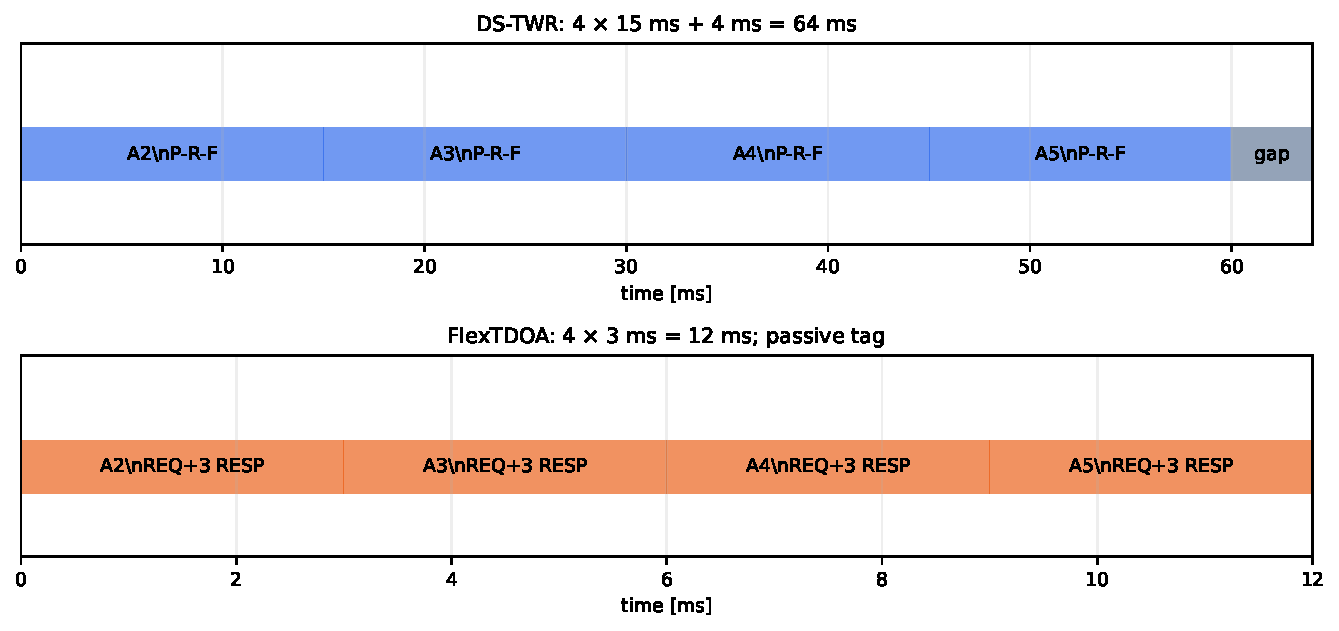
\includegraphics[width=\textwidth]{09_protocol_timing.pdf}
  \caption{Programarea temporală activă în test. P-R-F =
  \texttt{POLL--RESP--FINAL}.}
\end{figure}

\begin{table}[H]
  \centering
  \caption{Diferențe structurale relevante pentru sistem.}
  \small
  \begin{tabularx}{\textwidth}{p{31mm}YY}
    \toprule
    Caracteristică & DS-TWR nativ & FlexTDOA\\
    \midrule
    Rol tag & Activ; transmite două din cele trei cadre pentru fiecare
      distanță & Pasiv radio; doar recepționează\\
    Observabilă & Distanță absolută tag--ancoră & Diferență de distanță între
      două ancore\\
    Cadre & 3 per distanță: POLL, RESP, FINAL & 1 REQ + până la 3 RESP per
      slot\\
    Scalare cu tag-uri & Traficul UWB crește cu numărul de tag-uri & Tag-uri
      suplimentare fără sloturi UWB suplimentare\\
    Solver în test & Trilaterație liniară pe Raspberry Pi & AlgMin 2D pe ESP32
      și reproducere offline\\
    Filtrare temporală & Nu & Nu\\
    Profil activ & 64 ms/cadru cu 4 ancore & 12 ms/cadru cu 4 sloturi\\
    \bottomrule
  \end{tabularx}
\end{table}

\section{Configurația testată}

\subsection{Geometrie și referință}

Ancorele au fost măsurate ca un pătrat cu latura de 3,000 m, cu abatere
de poziționare declarată de maximum $\pm2$ mm. Convenția folosită în analiza
comună este:

\[
 A2=(0,0),\quad A3=(0,3),\quad A4=(3,0),\quad A5=(3,3)\ {\rm m},
\]
\[
 \mathbf p_{\rm tag}=(1{,}5;\,1{,}5)\ {\rm m}.
\]

Distanța adevărată tag--ancoră este aceeași pentru toate ancorele:

\[
 d_{\text{adevărat}}=\sqrt{1{,}5^2+1{,}5^2}
 =2{,}121320344\ {\rm m}.
\]

În centru, toate diferențele TDOA adevărate sunt zero. Această proprietate
permite evaluarea directă a fiecărui $z_{ij}$, fără a introduce eroarea unui
solver în analiza de măsurare.

\begin{figure}[H]
  \centering
  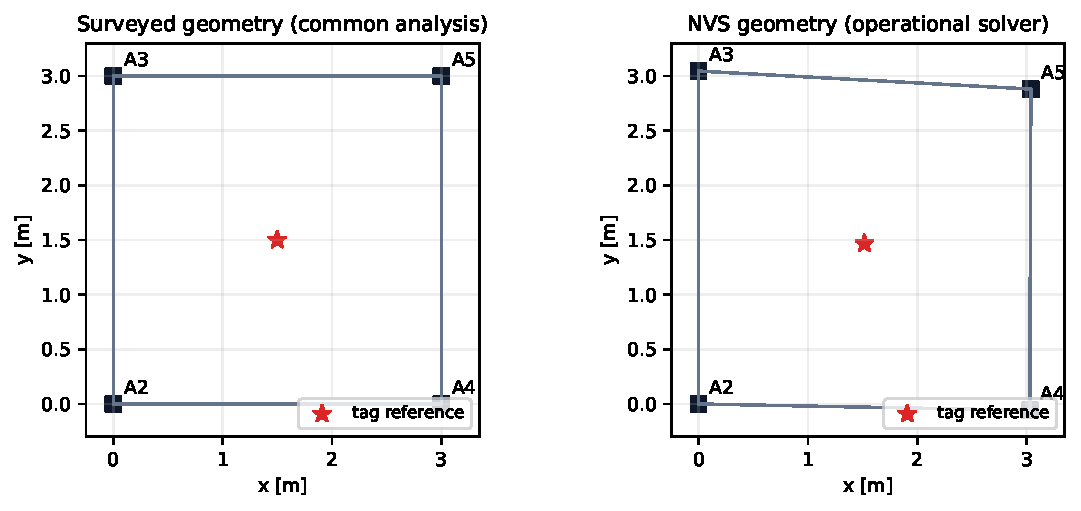
\includegraphics[width=0.86\textwidth]{01_geometry.pdf}
  \caption{Geometria măsurată folosită pentru comparația comună și geometria
  NVS utilizată de solverul operațional.}
\end{figure}

Geometria fixă aflată în NVS în momentul testului era:

\begin{center}
\begin{tabular}{lrrr}
  \toprule
  Ancoră & Coordonată NVS [m] & Coordonată măsurată [m] & Diferență [mm]\\
  \midrule
  A2 & $(0,000,\ 0,000)$ & $(0,000,\ 0,000)$ & $(0,\ 0)$\\
  A3 & $(0,000,\ 3,045)$ & $(0,000,\ 3,000)$ & $(0,\ +45)$\\
  A4 & $(3,030,\ -0,058)$ & $(3,000,\ 0,000)$ & $(+30,\ -58)$\\
  A5 & $(3,040,\ 2,880)$ & $(3,000,\ 3,000)$ & $(+40,\ -120)$\\
  \bottomrule
\end{tabular}
\end{center}

Prin urmare, pozițiile embedded FlexTDOA au fost evaluate în cadrul lor
operațional față de centrul geometriei NVS,
$(1,5175,\ 1,46675)$ m. Pentru comparația pură între protocoale, ambele soluții
offline folosesc pătratul măsurat și referința $(1,5,\ 1,5)$ m. Separarea
împiedică atribuirea erorii de auto-localizare a ancorelor protocolului de
poziționare.

\subsection{Parametri radio și temporali}

Ambele protocoale au folosit același hardware DW3000, canalul 5, 6,8 Mb/s,
PRF 64 MHz și preambul 128. Familia DW3000 este proiectată pentru TWR și TDoA,
iar producătorul declară o acuratețe de ranging sub 10 cm în specificația de
produs~\cite{qorvo-product,dwm3000-datasheet}; rezultatul prezentului raport se
referă însă numai la platforma și mediul concrete.

\begin{table}[H]
  \centering
  \caption{Profilurile runtime active, citite de la toate cele cinci module.}
  \small
  \begin{tabularx}{\textwidth}{lR{25mm}Y}
    \toprule
    Parametru & Valoare & Interpretare\\
    \midrule
    DS slot & 15 ms & buget pentru un schimb nativ\\
    DS gap după 4 ancore & 4 ms & cadru complet $4\times15+4=64$ ms\\
    DS RX slice / timeout & 100 / 8 ms & ascultare ancoră / timeout cadru așteptat\\
    DS RESP / FINAL delay & 2 / 2 ms & delayed-TX hardware\\
    DS auto-RX delay & 500 UUS & deschiderea RX după TX\\
    \midrule
    Flex guard & 250 $\mu$s & gardă pe slot\\
    Flex REQ subslot / process & 250 / 1.000 $\mu$s & cerere și procesare\\
    Flex RESP subslot & 250 $\mu$s & distanță între răspunsuri\\
    Flex process per responder & 250 $\mu$s & $3\times250\ \mu$s\\
    Flex slot / cadru & 3 / 12 ms & 333,33 sloturi/s; 83,33 cadre/s\\
    \bottomrule
  \end{tabularx}
\end{table}

Întârzierile de antenă active, în unitățile registrului DW3000, au fost:
M1 16.363, M2 16.368, M3 16.362, M4 16.371 și M5 16.371.

\section{Metodologie}

\subsection{Plan experimental}

\begin{itemize}[leftmargin=6mm]
  \item șase blocuri de câte 120 s, alternate Flex--DS pentru a reduce
  confundarea protocolului cu driftul termic sau temporal;
  \item 15 s de warm-up după fiecare schimbare de mod;
  \item polling dashboard la 50 Hz și deduplicare după ID de eveniment,
  secvență, slot și pereche;
  \item status complet la 1 Hz; toate cele cinci module au rămas online și în
  modul așteptat;
  \item zero erori de polling în toate cele șase blocuri;
  \item la final, sistemul a rămas în modul DS-TWR.
\end{itemize}

\subsection{Trei evaluări de poziție}

\paragraph{DS-TWR offline, geometrie măsurată.}
O poziție este calculată numai când există câte o distanță pentru A2--A5 din
același cadru. S-a folosit aceeași trilaterație liniară neponderată ca în
dashboard. Nu s-au eliminat distanțe pe baza amplitudinii erorii.

\paragraph{FlexTDOA offline, geometrie măsurată.}
Un slot este rezolvat numai când tag-ul a recepționat toți cei trei responderi.
AlgMin 2D reproduce convenția și iterațiile solverului din dashboard, pornind
determinist din centrul pătratului. Fiecare soluție folosește doar acel slot;
nu există seed temporal, medie sau filtrare.

\paragraph{FlexTDOA embedded, geometrie operațională.}
Sunt analizate direct pozițiile publicate de ESP32-S3. Acestea folosesc până la
12 diferențe direcționate recente și geometria NVS. Este seria relevantă pentru
ce vede utilizatorul în dashboard.

\subsection{Indicatori}

Raportăm bias pe axe, eroare radială mediană, P95, P99, maxim, RMSE 2D și
precizia față de centroidul eșantioanelor (CEP50/CEP95). Pentru măsurători
raportăm bias, deviație standard, MAE, P95 absolut și o deviație robustă
$1,4826\times{\rm MAD}$. Aceasta din urmă este necesară deoarece patru
observații FlexTDOA fizic imposibile ar distorsiona puternic deviația standard.

Repetabilitatea este evaluată pe cele trei blocuri, nu prin tratarea sutelor de
mii de eșantioane temporal corelate drept observații independente. Unde este
indicată o incertitudine 95\%, aceasta este intervalul Student al mediei celor
trei blocuri ($t_{0,975,2}=4,303$). Cu doar trei blocuri, intervalul trebuie
interpretat descriptiv.

\section{Rezultate}

\subsection{Debit, disponibilitate și rată de poziție}

\begin{table}[H]
  \centering
  \caption{Rezultate pe bloc. Pentru Flex, „complet” înseamnă trei răspunsuri
  distincte în slot; pentru DS, patru distanțe în cadrul de poziție. Poziția
  Flex este ieșirea embedded.}
  \scriptsize
  \begin{tabular}{lrrrrrr}
    \toprule
    Bloc & Măsurători & Măsurători/s & Livrare teoretică & Complet & Poziții/s &
      Mediană / P95\\
    \midrule
    Flex 1 & 95.932 & 799,07 & 79,91\% & 40,82\% & 25,66 & 3,72 / 7,56 cm\\
    DS 1   & 7.426  & 61,88  & 99,01\% & 97,70\% & 15,21 & 3,05 / 4,84 cm\\
    Flex 2 & 96.810 & 806,70 & 80,67\% & 43,01\% & 24,95 & 3,56 / 7,57 cm\\
    DS 2   & 7.400  & 61,66  & 98,66\% & 96,41\% & 15,01 & 3,05 / 4,83 cm\\
    Flex 3 & 96.974 & 807,97 & 80,80\% & 43,45\% & 25,00 & 3,49 / 7,52 cm\\
    DS 3   & 7.430  & 61,91  & 99,06\% & 97,91\% & 15,24 & 3,01 / 4,73 cm\\
    \bottomrule
  \end{tabular}
\end{table}

Media pe blocuri a fost:

\begin{itemize}[leftmargin=6mm]
  \item DS-TWR: $61,82\pm0,34$ distanțe/s și
  $15,15\pm0,31$ cadre complete/s (95\%);
  \item FlexTDOA: $804,58\pm11,96$ observații/s,
  $141,30\pm11,68$ sloturi complete rezolvabile/s și
  $25,20\pm0,99$ poziții embedded/s (95\%);
  \item rata observațiilor Flex a fost de 13,0 ori rata distanțelor DS;
  rata sloturilor Flex complete a fost de 9,3 ori rata cadrelor DS complete;
  ieșirea embedded efectivă a fost de 1,66 ori mai rapidă decât poziția DS.
\end{itemize}

Livrarea DS a fost 98,91\% din maximul profilului, iar 97,34\% dintre cadrele
candidate reconstruite au avut toate cele patru distanțe. La Flex, tag-ul a
observat 80,46\% din maximumul teoretic de 1.000 diferențe/s; 42,43\% dintre
sloturi au conținut toți cei trei responderi. Un solver rolling poate totuși
publica poziții folosind perechile recente, de aceea procentul de sloturi
complete nu este identic cu disponibilitatea poziției embedded.

\begin{figure}[H]
  \centering
  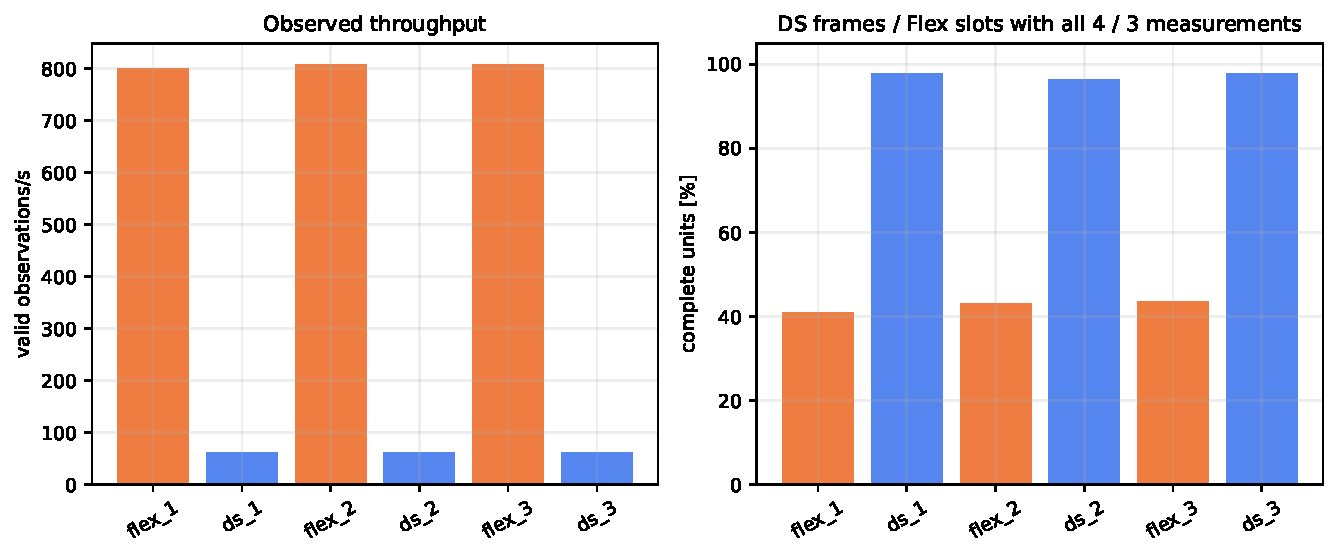
\includegraphics[width=0.94\textwidth]{07_throughput_completeness.pdf}
  \caption{Debitul observat și completitudinea unităților de poziție. Axele de
  debit compară observabile diferite: distanțe absolute DS și diferențe Flex.}
\end{figure}

\subsection{Calitatea măsurătorilor DS-TWR}

\begin{table}[H]
  \centering
  \caption{Eroarea distanței DS-TWR față de 2,121320344 m.}
  \small
  \begin{tabular}{lrrrrrr}
    \toprule
    Ancoră & $N$ & Bias & $\sigma$ & $\sigma_{\rm MAD}$ & MAE & P95 absolut\\
    \midrule
    A2 & 5.561 & +2,45 cm & 1,77 cm & 1,78 cm & 2,56 cm & 5,37 cm\\
    A3 & 5.555 & +8,02 cm & 0,92 cm & 0,89 cm & 8,02 cm & 9,77 cm\\
    A4 & 5.571 & +3,03 cm & 1,53 cm & 1,63 cm & 3,04 cm & 5,47 cm\\
    A5 & 5.569 & $-4,21$ cm & 1,56 cm & 1,48 cm & 4,22 cm & 6,53 cm\\
    \bottomrule
  \end{tabular}
\end{table}

DS-TWR are dispersie mică pe fiecare legătură, dar bias-ul este dependent de
modul: de la $-4,21$ cm la A5 până la $+8,02$ cm la A3. Aceasta indică o
oportunitate clară de recalibrare per modul/antenă. Bias-urile opuse se
proiectează parțial favorabil în poziția centrală; rezultatul de poziție nu
trebuie interpretat ca dovadă că fiecare distanță este calibrată la 3 cm.

\begin{figure}[H]
  \centering
  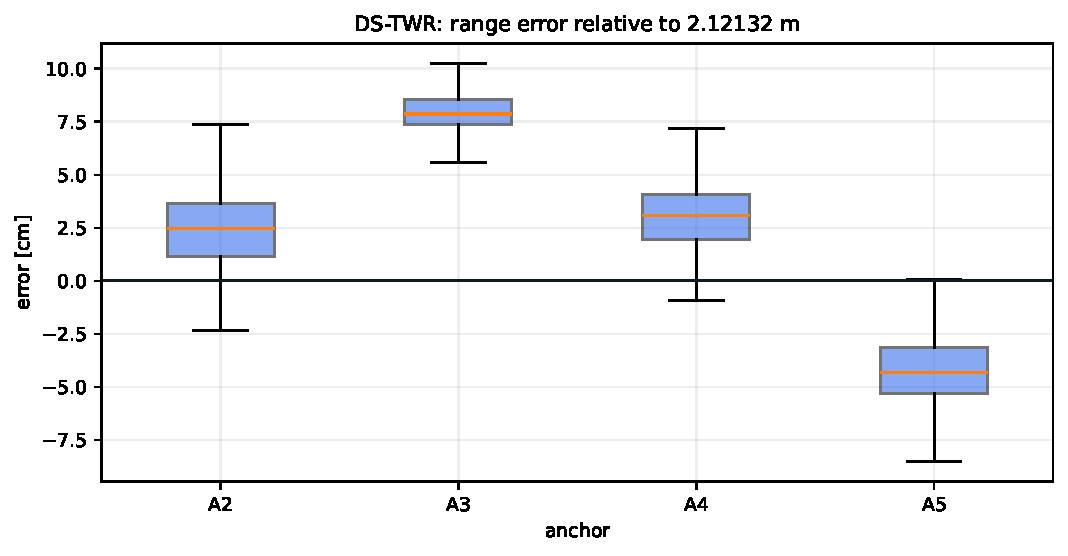
\includegraphics[width=0.78\textwidth]{02_ds_range_error.pdf}
  \caption{Distribuția nefiltrată a erorilor DS-TWR. Outlierii nu sunt desenați
  în boxplot, dar sunt incluși în toate metricile. Maximul absolut a fost
  11,47 cm.}
\end{figure}

\subsection{Calitatea observațiilor FlexTDOA}

La centru, valoarea adevărată pentru fiecare pereche direcționată este zero.
Corecția CFO + propagare anchor--anchor este esențială:

\begin{table}[H]
  \centering
  \caption{Toate cele 289.716 observații FlexTDOA, agregate. Bias-ul global
  corectat aproape zero include anularea bias-urilor direcționate și nu trebuie
  citit singur.}
  \small
  \begin{tabular}{lrrrrrr}
    \toprule
    Serie & Bias & $\sigma_{\rm MAD}$ & MAE & P95 abs. & P99 abs. & Maxim abs.\\
    \midrule
    Corectată & 0,13 cm & 12,31 cm & 10,05 cm & 24,10 cm & 36,40 cm &
      7.974,3 cm\\
    Necorectată & 71,89 cm & 35,43 cm & 72,03 cm & 122,40 cm & 131,40 cm &
      8.079,9 cm\\
    \bottomrule
  \end{tabular}
\end{table}

Pe perechi, bias-ul corectat se află între $-12,84$ și $+13,18$ cm, iar
dispersia robustă între 7,71 și 9,34 cm. Corecția reduce drastic offset-ul
normal, dar nu elimină cozile distribuției.

Au existat exact patru observații corectate care încalcă inegalitatea fizică
$|z_{ij}|\leq\|\mathbf a_i-\mathbf a_j\|+1$ cm: două în Flex 2 și două în
Flex 3, toate cu inițiator A3, în două sloturi izolate. Valorile au fost
aproximativ 79,6--79,7 m. Acest tipar este compatibil cu o discontinuitate de
timestamp sau de compensare a reply-ului, dar captura nu permite atribuirea
fără echivoc a cauzei interne. Rata este 4 din 289.716, adică 0,00138\%.

\begin{figure}[H]
  \centering
  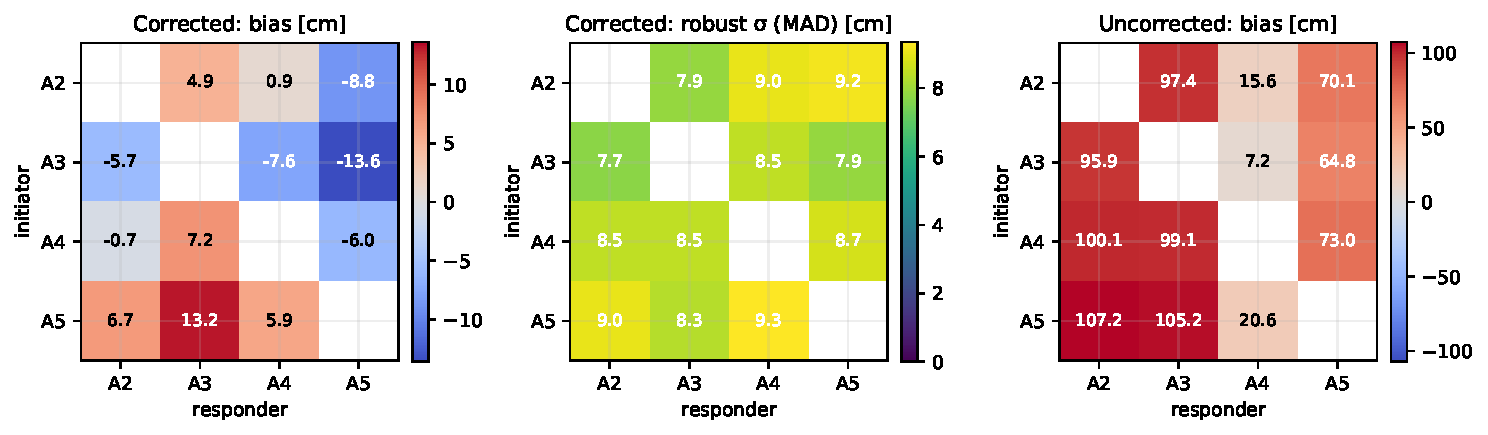
\includegraphics[width=\textwidth]{03_flex_pair_heatmaps.pdf}
  \caption{Bias și dispersie robustă pe perechi direcționate. Câmpul raw
  necorectat conține în principal reply delay-ul și offset-ul de ceas.}
\end{figure}

\subsection{Acuratețea poziției}

\begin{table}[H]
  \centering
  \caption{Metrici agregate de poziție. CEP este calculat față de centroidul
  propriei distribuții și descrie precizia, nu acuratețea absolută.}
  \scriptsize
  \begin{tabular}{lrrrrrrrr}
    \toprule
    Serie & Bias $x/y$ & RMSE & Mediană & P95 & P99 & CEP50/95 &
      $>50$ cm\\
    \midrule
    DS, geometrie măsurată &
      $+2,63/-0,99$ cm & 3,25 & 3,04 & 4,80 & 5,51 &
      1,35 / 2,78 cm & 0 / 5.455\\
    Flex, slot complet offline &
      $+4,53/+0,60$ cm & 9,94 & 7,64 & 17,17 & 25,50 &
      6,44 / 15,42 cm & 53 / 50.879\\
    Flex, ESP32 operațional &
      $+2,20/+0,47$ cm & 12,06 & 3,59 & 7,56 & 10,51 &
      2,85 / 6,64 cm & 1 / 9.075\\
    \bottomrule
  \end{tabular}
\end{table}

DS-TWR a fost mai precis și mai exact în comparația brută pe geometria
măsurată. Față de DS, FlexTDOA pe slot individual a avut RMSE de 3,06 ori mai
mare și P95 de 3,58 ori mai mare, dar a oferit de 9,3 ori mai multe sloturi
complete rezolvabile pe secundă.

Solverul embedded FlexTDOA este semnificativ mai stabil decât soluția unui
singur slot deoarece folosește mai multe perechi recente: P95 7,56 cm și,
în regimul sub 50 cm, RMSE 4,44 cm. P95 este de 1,58 ori valoarea DS, iar
RMSE-ul normal este de 1,37 ori valoarea DS. Acest câștig nu este rezultatul
unui filtru temporal explicit; provine din overdetermination și reutilizarea
setului curent de observații.

\begin{figure}[H]
  \centering
  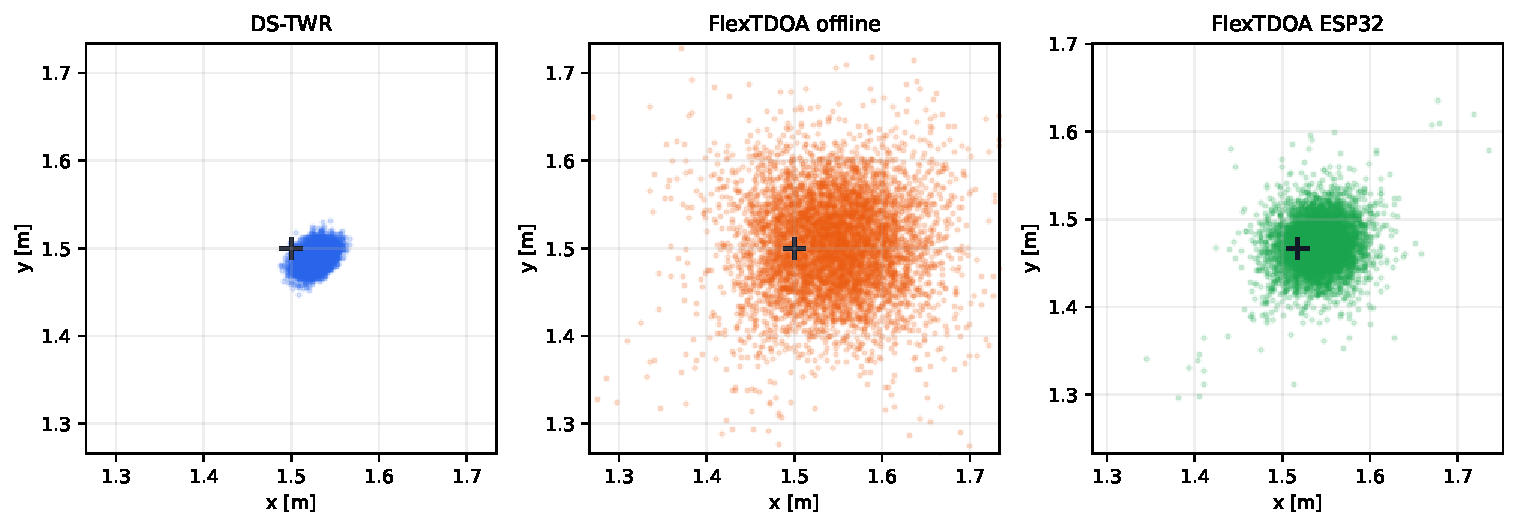
\includegraphics[width=\textwidth]{04_position_clouds.pdf}
  \caption{Norii de poziție. Crucea este referința corespunzătoare cadrului
  geometric. Graficul este limitat în jurul centrului pentru a arăta
  distribuția normală; evenimentul embedded de 10,68 m nu apare în fereastră.}
\end{figure}

\begin{figure}[H]
  \centering
  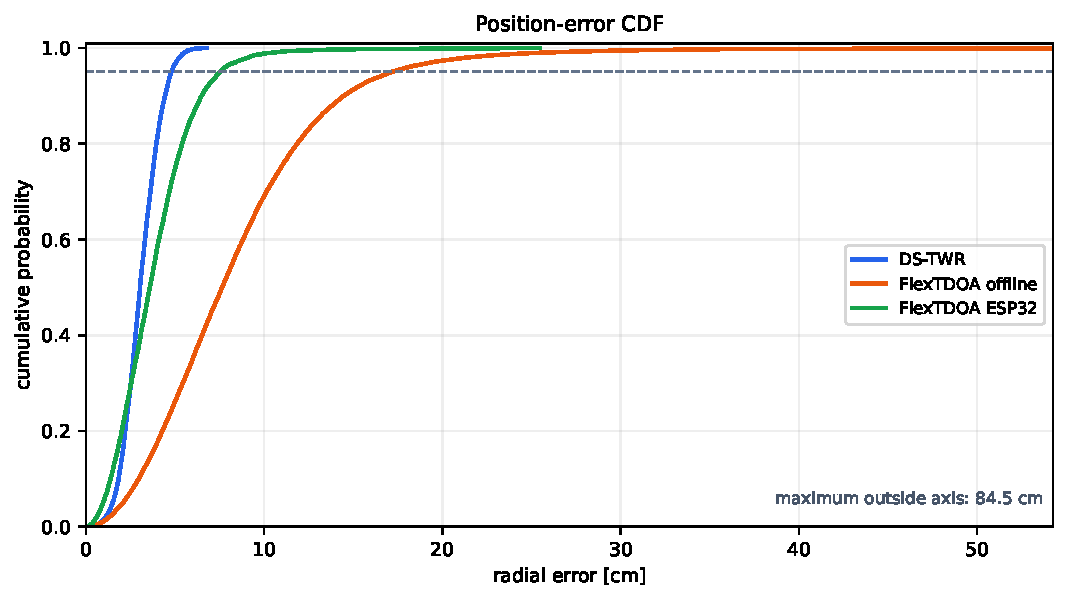
\includegraphics[width=0.85\textwidth]{05_position_error_cdf.pdf}
  \caption{Distribuția cumulată a erorii radiale, folosind toate eșantioanele.
  Limita axei este robustă; maximul din afara axei este notat în grafic.}
\end{figure}

\subsection{Evenimentul FlexTDOA catastrofal}

În Flex 2, slotul 26.933 a produs două observații de circa 79,6 și 79,7 m.
Solverul embedded a publicat o singură poziție
$(-6,364,\ 8,677)$ m, cu eroare 10,682 m și cu propriul indicator
\texttt{rms\_m}=21,854 m. Poziția embedded anterioară era
$(1,515,\ 1,454)$ m, iar următoarea a revenit la
$(1,555,\ 1,485)$ m. Evenimentul a durat deci un singur update publicat.

Fără eliminarea acestui punct, RMSE-ul Flex embedded pe toate blocurile este
12,06 cm. Pentru cele 9.074 poziții cu eroare sub 50 cm, RMSE este 4,44 cm.
P95 și P99 rămân 7,56 și 10,51 cm. Raportarea numai a RMSE ar descrie
incorect performanța obișnuită; raportarea numai a medianei ar ascunde un risc
operațional real.

O validare \emph{structurală}, nu un filtru de netezire, ar fi suficientă pentru
acest caz:

\[
 |z_{ij}| \leq \|\mathbf a_i-\mathbf a_j\|+\varepsilon,
\]

urmată de refuzul publicării unei poziții cu RMS intern incompatibil cu
geometria sau în afara unei limite operaționale. Aceasta nu modifică protocolul
FlexTDOA și nu inventează date; respinge o observație imposibilă fizic.

\subsection{Repetabilitate temporală}

DS-TWR a avut RMSE pe bloc de 3,20--3,28 cm și P95 de 4,73--4,84 cm. Media
RMSE pe bloc este $3,248\pm0,095$ cm (95\%). Flex offline a avut RMSE
9,90--10,01 cm și P95 16,96--17,34 cm, cu media RMSE
$9,940\pm0,154$ cm. Pentru Flex embedded, P95 a rămas remarcabil de stabil,
7,52--7,57 cm, deși RMSE-ul blocului 2 a fost afectat de evenimentul unic.

\begin{figure}[H]
  \centering
  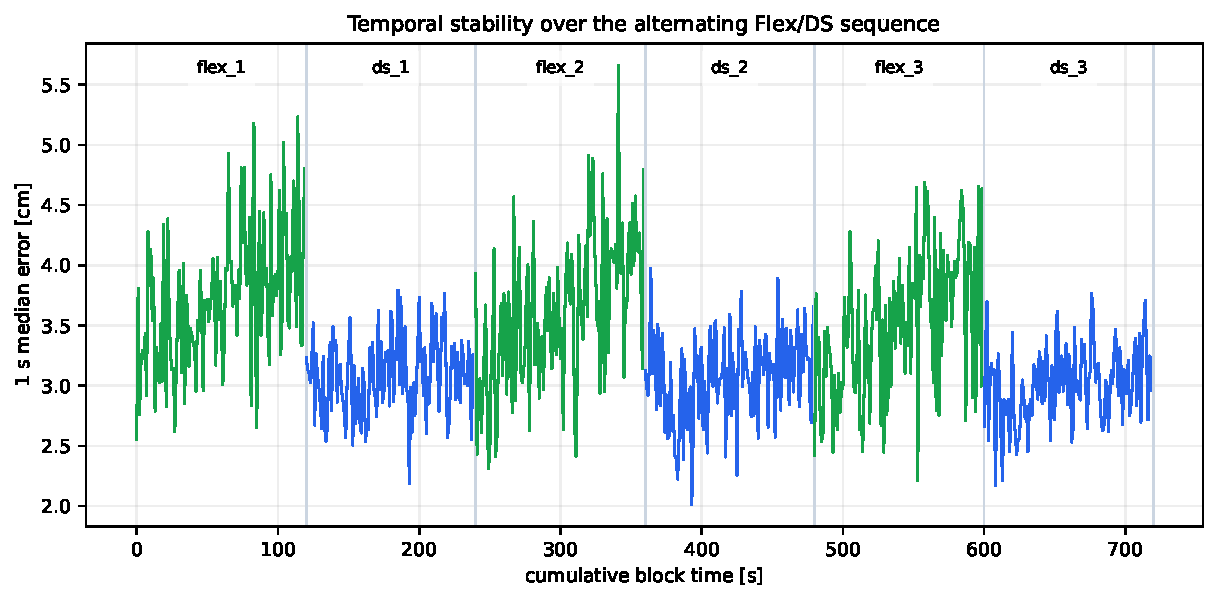
\includegraphics[width=\textwidth]{06_position_error_time.pdf}
  \caption{Mediana erorii pe intervale de 1 s. Evenimentele singulare nu sunt
  vizibile într-o mediană pe secundă și sunt analizate separat.}
\end{figure}

\begin{figure}[H]
  \centering
  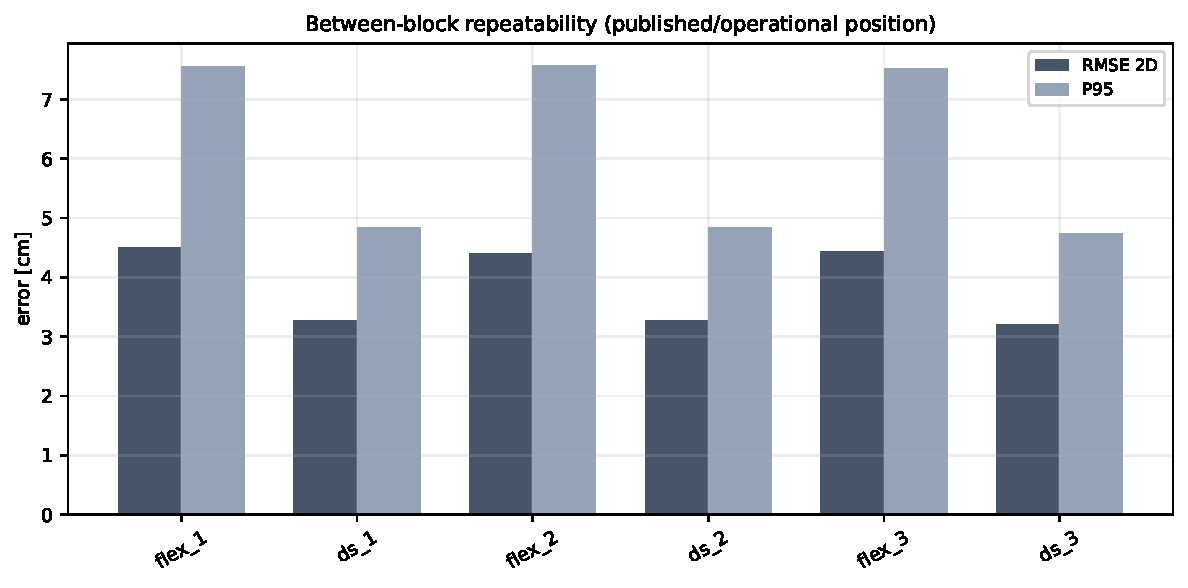
\includegraphics[width=0.88\textwidth]{08_block_repeatability.pdf}
  \caption{RMSE și P95 pe bloc pentru ieșirea operațională: DS offline și
  Flex embedded. Disocierea RMSE/P95 din Flex 2 evidențiază outlierul unic.}
\end{figure}

\section{Interpretare și alegerea protocolului}

\subsection{Când DS-TWR este alegerea potrivită}

\begin{itemize}[leftmargin=6mm]
  \item un tag sau puține tag-uri, unde traficul suplimentar este acceptabil;
  \item prioritate pe acuratețe și cozi scurte ale distribuției;
  \item este acceptabil ca tag-ul să transmită și să consume energie radio;
  \item o rată de circa 15 poziții/s satisface dinamica aplicației.
\end{itemize}

În testul actual, DS are cea mai bună combinație de RMSE, P95, stabilitate între
blocuri și completitudine a cadrului. Bias-ul per ancoră arată totuși că o
recalibrare poate îmbunătăți și mai mult acuratețea sau o poate schimba în alte
poziții.

\subsection{Când FlexTDOA este alegerea potrivită}

\begin{itemize}[leftmargin=6mm]
  \item tag complet pasiv în UWB și autonomie/scalabilitate prioritare;
  \item mai multe tag-uri care trebuie localizate fără a consuma sloturi
  suplimentare;
  \item rată mare a observațiilor și actualizare mai rapidă;
  \item aplicația tolerează P95 de circa 7,6 cm în configurația curentă și
  implementează validarea ieșirilor imposibile.
\end{itemize}

FlexTDOA nu este doar „DS mai rapid”; observabila, topologia și costul de
scalare sunt diferite. La patru ancore, profilul de 12 ms produce 83,33 cadre/s
și 333,33 sloturi/s, independent de numărul de tag-uri pasive. Pentru o
instalație cu mai multe tag-uri, comparația de airtime devine progresiv mai
favorabilă FlexTDOA.

\subsection{Recomandări imediate}

\begin{enumerate}[leftmargin=7mm]
  \item Păstrarea DS-TWR nativ fără filtru, cu profilul de 64 ms, ca baseline
  de acuratețe.
  \item Recalibrarea întârzierilor de antenă, în special pentru legăturile A3
  și A5; apoi repetarea exactă a testului.
  \item Scrierea geometriei măsurate în NVS înaintea comparațiilor
  operaționale; geometria curentă diferă până la 12 cm pe axa $y$.
  \item Pentru FlexTDOA, adăugarea porții fizice
  $|z_{ij}|\leq d_{ij}+\varepsilon$ și a unui quality gate pe RMS/bounding box.
  Acestea sunt verificări de validitate, nu filtrare temporală.
  \item Repetarea pe o grilă de minimum 5×5 puncte, inclusiv margini și
  exteriorul pătratului, apoi test dinamic și NLOS. Centrul singur nu
  caracterizează GDOP-ul întregii suprafețe.
  \item Pentru mișcare, raportarea latenței end-to-end cu timestamp hardware,
  nu doar a ratei de evenimente recepționate de dashboard.
\end{enumerate}

\section{Limitări}

\begin{itemize}[leftmargin=6mm]
  \item Un singur punct, static și central; nu poate descrie erorile spațiale.
  \item Test LOS; NLOS și multipath sever nu sunt reprezentate.
  \item Geometria este declarată la $\pm2$ mm, dar nu a fost inclus un sistem
  optic extern sau o stație totală în captura digitală.
  \item Temperatura și RSSI au fost înregistrate, dar nu au fost variate
  controlat.
  \item Poziția DS este calculată pe Raspberry Pi, iar poziția Flex operațională
  pe ESP32; de aceea raportul include și o soluție Flex offline comună.
  \item Debitul observat prin telemetrie/dashboard este o limită
  end-to-end a implementării, nu doar capacitatea PHY a protocolului.
  \item Setul provine din firmware \texttt{-dirty}; manifestul și commit-ul
  permit identificarea, dar reproducerea exactă necesită păstrarea modificărilor
  locale curente.
\end{itemize}

\section{Concluzie}

În configurația măsurată $3\times3$ m, tag central, LOS:

\begin{itemize}[leftmargin=6mm]
  \item \textbf{DS-TWR câștigă la acuratețe și predictibilitate}: RMSE
  3,25 cm, mediană 3,04 cm, P95 4,80 cm, fără erori peste 6,79 cm în pozițiile
  complete;
  \item \textbf{FlexTDOA câștigă la debit și scalabilitate}: 804,6
  observații/s, tag radio-pasiv și 25,2 poziții embedded/s;
  \item \textbf{FlexTDOA embedded este bun în regim normal}, cu mediană
  3,59 cm, P95 7,56 cm și RMSE 4,44 cm sub pragul de 50 cm;
  \item \textbf{FlexTDOA are nevoie de o gardă structurală}: o poziție din
  9.075 a avut eroare 10,68 m, provocată de observații imposibile fizic;
  \item \textbf{alegerea depinde de produs}: DS pentru acuratețe cu puține
  tag-uri; FlexTDOA pentru tag pasiv, multe tag-uri și rată mare.
\end{itemize}

Aceste concluzii sunt solide pentru testul efectuat datorită alternării
blocurilor, volumului mare de date și stabilității inter-bloc, dar următorul
pas obligatoriu pentru o alegere de sistem este harta spațială LOS/NLOS.

\clearpage
\appendix

\begin{landscape}
\section{Metrici FlexTDOA pe perechi direcționate}

\scriptsize
\begin{longtable}{lrrrrrrr}
  \caption{Observații FlexTDOA corectate; adevărul este 0 m pentru tag-ul
  central. $\sigma_{\rm MAD}=1,4826\times{\rm MAD}$.}\\
  \toprule
  Pereche & $N$ & Bias [cm] & $\sigma_{\rm MAD}$ [cm] & P95 abs. [cm] &
  P99 abs. [cm] & Maxim abs. [cm] & Imposibile fizic\\
  \midrule
  \endfirsthead
  \toprule
  Pereche & $N$ & Bias [cm] & $\sigma_{\rm MAD}$ [cm] & P95 abs. [cm] &
  P99 abs. [cm] & Maxim abs. [cm] & Imposibile fizic\\
  \midrule
  \endhead
  A2$\to$A3 & 25.583 & +4,92 & 7,86 & 20,00 & 30,60 & 101,60 & 0\\
  A2$\to$A4 & 25.192 & +0,89 & 9,04 & 20,00 & 31,21 & 108,60 & 0\\
  A2$\to$A5 & 24.354 & $-8,80$ & 9,19 & 26,40 & 52,75 & 211,40 & 0\\
  A3$\to$A2 & 23.517 & $-5,37$ & 7,71 & 21,20 & 36,37 & 7.968,70 & 1\\
  A3$\to$A4 & 22.518 & $-7,29$ & 8,45 & 23,10 & 34,20 & 7.963,60 & 1\\
  A3$\to$A5 & 20.734 & $-12,84$ & 7,86 & 27,90 & 37,90 & 7.974,30 & 2\\
  A4$\to$A2 & 24.892 & $-0,69$ & 8,45 & 18,90 & 30,80 & 93,60 & 0\\
  A4$\to$A3 & 24.316 & +7,18 & 8,45 & 23,10 & 35,49 & 104,40 & 0\\
  A4$\to$A5 & 23.612 & $-5,98$ & 8,75 & 22,10 & 33,30 & 100,80 & 0\\
  A5$\to$A2 & 24.976 & +6,73 & 9,04 & 24,90 & 42,20 & 177,40 & 0\\
  A5$\to$A3 & 24.931 & +13,18 & 8,30 & 28,55 & 37,77 & 124,10 & 0\\
  A5$\to$A4 & 25.091 & +5,87 & 9,34 & 23,20 & 34,50 & 107,80 & 0\\
  \bottomrule
\end{longtable}
\end{landscape}

\section{Fișiere și reproducere}

Artefactele sunt păstrate în:
\begin{quote}
\path{/home/pi/Documents/UWB/reports/uwb_protocol_comparison_20260726}
\end{quote}

\small
\noindent
\begin{tabularx}{\textwidth}{p{56mm}Y}
  \toprule
  Fișier/director & Conținut\\
  \midrule
  \path{data/*.jsonl} & capturile brute, un fișier per bloc\\
  \path{data/*.metadata.json} & configurația, statusul și contoarele fiecărui
  bloc\\
  \path{raw_data_manifest.csv} & dimensiune și SHA-256 pentru fiecare
  fișier brut\\
  \path{analysis_summary.json} & toate metricile agregate\\
  \path{measurement_metrics.csv} & metrici per ancoră/pereche\\
  \path{position_metrics.csv} & metrici de poziție agregate\\
  \path{block_metrics.csv} & rezultate pe cele șase blocuri\\
  \path{ds_positions.csv} & poziții DS reconstruite\\
  \path{flex_slot_positions.csv} & poziții Flex pe slot complet\\
  \path{flex_embedded_positions.csv} & poziții publicate de ESP32\\
  \path{figures/} & toate graficele, PDF vectorial și PNG\\
  \bottomrule
\end{tabularx}

\paragraph{Reproducerea analizei}
\begin{verbatim}
cd /home/pi/Documents/UWB
python3 tools/uwb_compare_analyze.py
cd reports/uwb_protocol_comparison_20260726
latexmk -pdf -interaction=nonstopmode -halt-on-error report.tex
\end{verbatim}

Scriptul de colectare este \path{tools/uwb_compare_collect.py}, iar scriptul de
analiză este \path{tools/uwb_compare_analyze.py}. Fișierele raw nu sunt
modificate de analiză.

\begin{thebibliography}{9}

\bibitem{flextdoa-paper}
G.-C. Pătru, L. Flueratoru, I. Vasilescu, D. Niculescu și D. Rosner,
``FlexTDOA: Robust and Scalable Time-Difference of Arrival Localization Using
Ultra-Wideband Devices,'' \emph{IEEE Access}, vol. 11, 2023,
pp. 28610--28627.
\href{https://doi.org/10.1109/ACCESS.2023.3259320}
{doi:10.1109/ACCESS.2023.3259320}.

\bibitem{qorvo-api}
Qorvo, \emph{DW3xxx Device Driver API Guide}, secțiunile 6.3.26--6.3.29,
exemplele double-sided two-way ranging, 2025.
\url{https://forum.qorvo.com/uploads/short-url/xD3TlXKvkujjdUaJWXv2b4E7GQN.pdf}.

\bibitem{aps013}
Decawave, \emph{APS013: DW1000 and Two-Way Ranging}, rev. 2.3,
Poll--Response--Final și formula asymmetric DS-TWR.
\url{https://forum.qorvo.com/uploads/short-url/x34DrF7EW5fQP9wY3aNESqPKz8z.pdf}.

\bibitem{qorvo-product}
Qorvo, \emph{DW3110 Ultra-Wideband Transceiver}, specificații și documentație
DW3000.
\url{https://www.qorvo.com/products/p/DW3110}.

\bibitem{dwm3000-datasheet}
Qorvo, \emph{DWM3000 IEEE 802.15.4-z UWB Transceiver Module Data Sheet},
rev. B, mai 2021. Copie locală:
\path{datasheets/DWM3000 Data Sheet.pdf}.

\bibitem{firmware}
Repository local \emph{UWB Module ESP-IDF}, commit
\texttt{a97cdce60d191360300f8f39e6afa77247a59f77}, ramura
\texttt{experiment/ds-twr-native-performance}, stare de lucru din
26 iulie 2026.

\end{thebibliography}

\end{document}
